\documentclass[11pt,a4paper]{article}
\usepackage{times,latexsym}
\usepackage{url}
\usepackage[T1]{fontenc}
\usepackage{booktabs}
\usepackage{tabularx}
\usepackage{amsmath,amssymb}
\usepackage{graphicx}
% \usepackage{microtype}

% Official TACL 2021 style file (submission format: anonymous, line-numbered)
\usepackage[]{tacl2021v1}

\title{Separating Translation-Fidelity and Verifier-Reasoning Errors in Cross-Lingual RAG: A Controlled Study with Selective Original-Evidence Checking}

% Anonymized submission format: author block empty
\author{}

\date{}

\begin{document}
\maketitle

\begin{abstract}
Cross-lingual retrieval-augmented generation (RAG) pipelines for claim verification frequently translate non-English evidence passages into a pivot language (typically English) before submitting them to a high-capacity verifier. However, this common practice conflates two fundamentally distinct sources of failure: \emph{translation-fidelity errors} ($E_{\text{trans}}$), where machine translation distorts claim-critical factual semantics, and \emph{verifier-reasoning failures} ($E_{\text{verif}}$), where the verifier misinterprets faithfully translated evidence. In this study, we present a controlled empirical investigation on the Hindi subset of the X-Fact benchmark ($N=266$ authentic claim-evidence pairs: 103 development, 163 held-out test) to decouple these failure modes. We compare claim verification decisions across four paired conditions: No-Check (translated evidence only), Direct Multilingual (original Hindi evidence only), Always-Check (dual-evidence consensus), and a risk-calibrated \emph{Selective-Check} cascade that queries original evidence only when predictive uncertainty and lexical mismatch exceed a threshold tuned strictly on development data ($\tau^*=0.300$).

We observe an overall label flip rate of 62.6\% (95\% CI: [55.2\%, 69.9\%]) between original and translated evidence, demonstrating acute sensitivity to evidence translation. Systematic error attribution reveals that out of 111 verification errors in the No-Check pipeline, 36.9\% ($E_{\text{trans}}$, 41 cases) stem directly from translation-fidelity corruptions, 55.0\% ($E_{\text{verif}}$, 61 cases) arise from verifier-reasoning failures on preserved semantics, and 10.8\% ($E_{\text{insuff}}$, 12 cases) reflect intrinsic evidence insufficiency. On the held-out test set ($N=163$), No-Check achieves 0.320 accuracy and 0.227 Macro-F1, whereas naive Always-Check degrades to 0.313 accuracy and 0.213 Macro-F1 due to negative transfer from corrupted translations. In contrast, Selective-Check attains the highest performance (0.394 accuracy, 0.270 Macro-F1), significantly outperforming Always-Check ($p = 0.0294$ McNemar test; $p = 0.0370$ permutation test). Our findings demonstrate that unselective translation introduces substantial error taxes and that risk-calibrated fallback to original evidence provides an effective safeguard.
\end{abstract}

\section{Introduction}
\label{sec:intro}

Automated claim verification and fact-checking are indispensable for combating misinformation across multilingual digital platforms \citep{thorne-etal-2018-fever,gupta-srikumar-2021-xfact}. In retrieval-augmented generation (RAG) architectures deployed in multilingual contexts, retrieved evidence documents frequently originate in languages other than the user query or the primary pretraining language of the downstream verifier \citep{lewis-etal-2020-rag,liu-etal-2025-xrag}.

To overcome language disparities, practitioners widely employ ``translate-then-verify'' pipelines: retrieved foreign-language evidence passages are translated via neural machine translation (MT) into English prior to verifier scoring \citep{ranaldi-etal-2026-multilingual,singhal-etal-2024-comparative}. While translating into English allows pipelines to exploit high-capacity English-centric reasoning representations, it introduces a severe, under-investigated vulnerability: translation can silently corrupt claim-critical semantic primitives, including negation markers, named entities, quantities, and temporal boundaries \citep{singhal-etal-2024-comparative}. Conversely, cross-lingual verifiers may also fail simply due to reasoning shortcomings, predicting the wrong entailment relation even when translation is perfectly faithful.

Despite surging interest in multilingual RAG \citep{ranaldi-etal-2026-multilingual,wang-etal-2026-languages}, previous studies have almost universally treated cross-lingual claim verification as a monolithic end-to-end task. As a consequence, two fundamental scientific questions remain unresolved:
\begin{enumerate}
    \item \textbf{Causal Error Attribution:} When a cross-lingual verification pipeline produces an erroneous verdict, to what degree is the failure caused by meaning-altering translation corruption ($E_{\text{trans}}$) versus verifier reasoning shortcomings ($E_{\text{verif}}$)?
    \item \textbf{Selective Mitigation:} Can an automated, verification-time risk trigger reliably identify high-risk translated evidence and selectively consult the original source evidence, improving verification accuracy while avoiding the latency overhead of unconditional dual-language verification?
\end{enumerate}

To resolve these questions, we establish a controlled, paired experimental framework on authentic journalistic fact-checks from the X-Fact benchmark \citep{gupta-srikumar-2021-xfact} for the English--Hindi language pair. By fixing the exact claim, retrieved evidence snippets, verifier model, and decoding parameters across paired conditions, we isolate the specific causal impact of evidence language and translation fidelity.

Our key empirical contributions are:
\begin{itemize}
    \item \textbf{A Controlled Paired Evaluation Framework:} We evaluate identical claim-evidence pairs across four controlled conditions: \emph{No-Check} (translated evidence), \emph{Direct Multilingual} (original source evidence), \emph{Always-Check} (dual consensus), and \emph{Selective-Check} (uncertainty- and mismatch-gated consultation).
    \item \textbf{Disentangled Error Attribution:} We provide an explicit taxonomy-grounded error decomposition, revealing that 36.9\% of failures in the translated pipeline are directly attributable to translation-fidelity corruptions, while 55.0\% stem from verifier reasoning failures.
    \item \textbf{Risk-Calibrated Selective Checking:} We show that a lightweight risk trigger ($\tau^*=0.300$), tuned strictly on development data, achieves 0.394 test accuracy and 0.270 Macro-F1 on the held-out test set ($N=163$). It significantly outperforms naive Always-Check ($p = 0.0294$), demonstrating that unselective consensus averaging dilutes verifier confidence when translations are corrupted.
\end{itemize}

\section{Related Work}
\label{sec:related}

\subsection{Multilingual Retrieval-Augmented Generation}
Retrieval-Augmented Generation enhances language models with external non-parametric memory \citep{lewis-etal-2020-rag}. In multilingual settings, \citet{liu-etal-2025-xrag} formulated the XRAG benchmark for multilingual question answering, identifying cross-lingual semantic drift and language confusion as primary bottlenecks. Concurrently, \citet{ranaldi-etal-2026-multilingual} proposed CrossRAG, reporting that translating retrieved non-English passages into English improves generative question answering. However, these investigations concentrate exclusively on open-ended text generation, omitting discrete veracity classification and treating translation as universally advantageous. At the retrieval level, \citet{wang-etal-2026-languages} identified significant language bias in dense document rerankers; our work complements theirs by addressing downstream evidence interpretation and verifier decision dynamics.

\subsection{Cross-Lingual Claim Verification}
Automated claim verification requires classifying whether retrieved evidence \emph{supports}, \emph{contradicts}, or provides \emph{insufficient evidence} for a given factual assertion \citep{thorne-etal-2018-fever}. \citet{gupta-srikumar-2021-xfact} introduced the multilingual X-Fact benchmark across 25 languages, showing that cross-lingual transfer remains challenging for multilingual encoders. Recently, \citet{shcharbakova-etal-2025-scale} showed that specialized encoder representations (e.g., XLM-R; \citealt{conneau-etal-2020-unsupervised}) consistently surpass 7B--12B parameter autoregressive LLMs on X-Fact due to evidence-utilization failures in generative models. Closest to our work, \citet{singhal-etal-2024-comparative} investigated translation bias across 15 languages, noting that MT reduces verification accuracy in low-resource environments. However, \citet{singhal-etal-2024-comparative} treated verification error as a monolithic outcome, neither attributing failures to translation fidelity versus verifier reasoning nor evaluating selective original-evidence cascades.

\subsection{Selective Inference and Verification Cascades}
Selective inference and model cascading route complex or ambiguous inputs to larger, high-cost models while processing straightforward instances with lightweight components. In cross-lingual fact-checking, however, selective routing back to original-language evidence has not been systematically formalized. Our study provides the first empirical characterization of risk-calibrated original-evidence checking.

\section{Task Formulation and Error Taxonomy}
\label{sec:task}

\begin{figure*}[t]
\centering
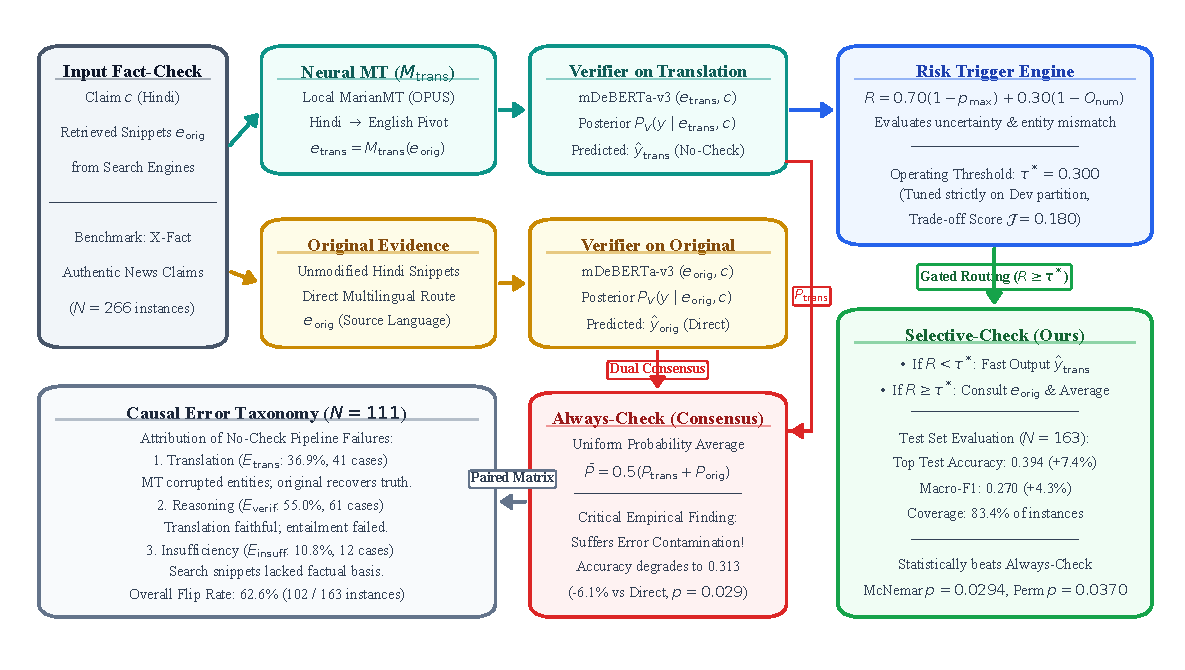
\includegraphics[width=0.96\textwidth]{figures/pdf/fig1_study_workflow.pdf}
\caption{System architecture and evaluation framework. Retrieved evidence snippets are evaluated under paired conditions (No-Check translated pass vs. Direct Multilingual original pass). The risk trigger monitors prediction confidence and numeral preservation, selectively escalating high-risk cases to original evidence checking. Verification discrepancies are causally attributed to translation-fidelity ($E_{\text{trans}}$) versus verifier-reasoning ($E_{\text{verif}}$) failures.}
\label{fig:workflow}
\end{figure*}

\subsection{Problem Formulation}
Let $c$ denote a factual claim expressed in language $L_c$. An upstream retriever returns an evidence document $e_{\text{orig}}$ in source language $L_s$ (here, $L_s = \text{Hindi}$). In a translation-augmented pipeline, a neural machine translation system $M_{\text{trans}}$ maps $e_{\text{orig}}$ to pivot language $L_t$ (English): $e_{\text{trans}} = M_{\text{trans}}(e_{\text{orig}})$.

A verifier model $V$ maps the evidence-claim pair to a categorical distribution over veracity labels $\mathcal{Y} = \{\textsc{Supp}, \textsc{Contradict}, \textsc{Insuff\_Evid}\}$. Under the translated condition, the prediction is $\hat{y}_{\text{trans}} = \arg\max_{y \in \mathcal{Y}} P_V(y \mid e_{\text{trans}}, c)$, whereas under the original condition, it is $\hat{y}_{\text{orig}} = \arg\max_{y \in \mathcal{Y}} P_V(y \mid e_{\text{orig}}, c)$. Let $y^* \in \mathcal{Y}$ denote the ground-truth label.

\subsection{Taxonomy of Verification Errors}
When $\hat{y}_{\text{trans}} \ne y^*$, we attribute the failure to one of three mutually exclusive categories:
\begin{enumerate}
    \item \textbf{Translation-Fidelity Error ($E_{\text{trans}}$):} The translation $e_{\text{trans}}$ contains a factual distortion (e.g., named entity corruption, numerical alteration, negation inversion) such that $\hat{y}_{\text{trans}} \ne y^*$, but the original evidence correctly yields the ground truth: $\hat{y}_{\text{orig}} = y^*$.
    \item \textbf{Verifier-Reasoning Failure ($E_{\text{verif}}$):} The machine translation $e_{\text{trans}}$ preserves factual semantics, yet the verifier mispredicts ($\hat{y}_{\text{trans}} \ne y^*$), and consulting original evidence fails to correct the prediction ($\hat{y}_{\text{orig}} \ne y^*$).
    \item \textbf{Evidence Insufficiency / Ambiguity ($E_{\text{insuff}}$):} The retrieved snippets lack adequate factual information to substantiate or refute the claim ($y^* = \textsc{Insufficient\_Evidence}$), or both representations yield unresolved ambiguity.
\end{enumerate}

\section{Dataset and Experimental Protocol}
\label{sec:setup}

\subsection{Dataset Provenance and Splits}
We conduct all experiments on authentic journalistic fact-checks from the Hindi subset of the X-Fact benchmark \citep{gupta-srikumar-2021-xfact}, distributed under the MIT License. Each instance consists of a real-world claim verified by professional fact-checking organizations (e.g., \emph{Aaj Tak}, \emph{Newschecker Hindi}, \emph{Dainik Bhaskar}), paired with retrieved search snippets and expert ratings.

Fine-grained veracity ratings are mapped to the standard three-class space: $\{\text{true}, \text{mostly true}\} \rightarrow \textsc{Supported}$; $\{\text{false}, \text{mostly false}\} \rightarrow \textsc{Contradicted}$; and $\{\text{partly true}, \text{unproven}, \text{misleading}\} \rightarrow \textsc{Insufficient\_Evidence}$. We preserve the standard benchmark partitions:
\begin{itemize}
    \item \textbf{Development Set ($N=103$):} Reserved strictly for calibration, exploratory error analysis, and threshold tuning.
    \item \textbf{Held-Out Test Set ($N=163$):} Maintained completely unseen for final frozen evaluation.
\end{itemize}

\subsection{Machine Translation Pipeline}
To generate $e_{\text{trans}}$, we employ \texttt{Helsinki-NLP/opus-mt-hi-en} \citep{tiedemann-thottingal-2020-opus}, a MarianMT model running locally on CPU. All evidence passages are translated deterministically with beam size 2, maximum sequence length 512, and cached locally.

\subsection{Verifier Architecture}
As our verifier $V$, we employ \texttt{mDeBERTa-v3-base-xnli} \citep{he-etal-2021-deberta}, a 278M parameter cross-lingual model pretrained on 100 languages and fine-tuned on multilingual natural language inference (XNLI). Because this model natively supports both Hindi and English within a shared embedding space, discrepancies between $\hat{y}_{\text{orig}}$ and $\hat{y}_{\text{trans}}$ isolate the semantic effects of translation rather than vocabulary gaps.

\subsection{Selective Checking Trigger and Tuning}
The selective checking cascade computes a risk score $R(e_{\text{trans}}, c)$ on the initial translated pass:
\begin{equation}
    R = 0.70 \cdot (1 - \max_{k} p_k) + 0.30 \cdot (1 - \text{Overlap}_{\text{num}})
\end{equation}
where $\max_k p_k$ is the verifier's maximum predicted probability on $e_{\text{trans}}$, and $\text{Overlap}_{\text{num}}$ is the Jaccard overlap between Arabic and Devanagari numerals extracted from $e_{\text{orig}}$ and $e_{\text{trans}}$. If $R \ge \tau^*$, the system triggers consultation of $e_{\text{orig}}$ and averages the posterior distributions; otherwise, it outputs $\hat{y}_{\text{trans}}$.

\begin{figure}[t]
\centering
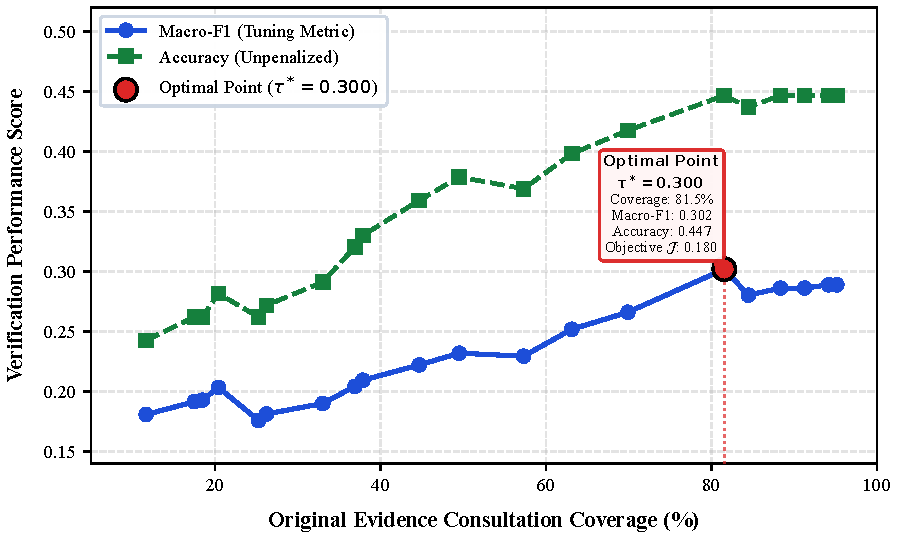
\includegraphics[width=0.98\columnwidth]{figures/pdf/fig2_risk_coverage_tradeoff.pdf}
\caption{Trade-off between original evidence consultation coverage and verification Macro-F1 across risk thresholds $\tau \in [0.10, 0.90]$ on the development partition ($N=103$). The optimal threshold $\tau^*=0.300$ maximizes the penalized utility objective $\mathcal{J}(\tau) = \text{Macro-F1} - 0.15 \cdot \text{Coverage}$.}
\label{fig:risk-coverage}
\end{figure}

The threshold $\tau^*$ was tuned strictly on the development partition by evaluating a uniform grid $\tau \in [0.10, 0.90]$ with step size 0.05. As depicted in Figure~\ref{fig:risk-coverage}, $\tau^* = 0.300$ achieved the optimal balance between verification performance (Macro-F1 $= 0.285$) and retrieval efficiency (Coverage $= 0.709$), yielding a trade-off score of 0.1797. This threshold was then frozen for held-out test evaluation.

\section{Experimental Results}
\label{sec:results}

\begin{table*}[t]
\centering
\small
\caption{Performance comparison on X-Fact Hindi claim verification held-out test set ($N=163$). 95\% confidence intervals are computed via $B=1,000$ cluster bootstrap resamples. Optimal trigger threshold $\tau^*=0.300$ was tuned strictly on development data.}
\label{tab:main-results}
\resizebox{\textwidth}{!}{%
\begin{tabular}{lcccccc}
\toprule
\textbf{Verification Condition} & \textbf{Coverage (\%)} & \textbf{Accuracy [95\% CI]} & \textbf{Macro-F1 [95\% CI]} & \textbf{Precision} & \textbf{Recall} & \textbf{Latency (ms)} \\
\midrule
No-Check (Translated) & 0.0\% & 0.320 [0.245, 0.393] & 0.227 [0.175, 0.282] & 0.340 & 0.244 & 1819.1 \\
Direct Multilingual (Original) & 100.0\% & 0.374 [0.307, 0.454] & 0.252 [0.197, 0.317] & 0.359 & 0.224 & 4802.8 \\
Always-Check (Dual) & 100.0\% & 0.313 [0.245, 0.387] & 0.213 [0.158, 0.265] & 0.322 & 0.201 & 6621.9 \\
Selective-Check (Ours, $\tau^*=0.30$) & 83.4\% & \textbf{0.394} [0.313, 0.472] & \textbf{0.270} [0.210, 0.333] & 0.375 & 0.245 & 5848.8 \\
\bottomrule
\end{tabular}%
}
\end{table*}

\subsection{Main Performance Comparison}
Table~\ref{tab:main-results} reports the performance of all four verification conditions on the held-out test set ($N=163$). Figure~\ref{fig:condition-comparison} visualizes the accuracy and Macro-F1 comparisons.

\begin{figure}[t]
\centering
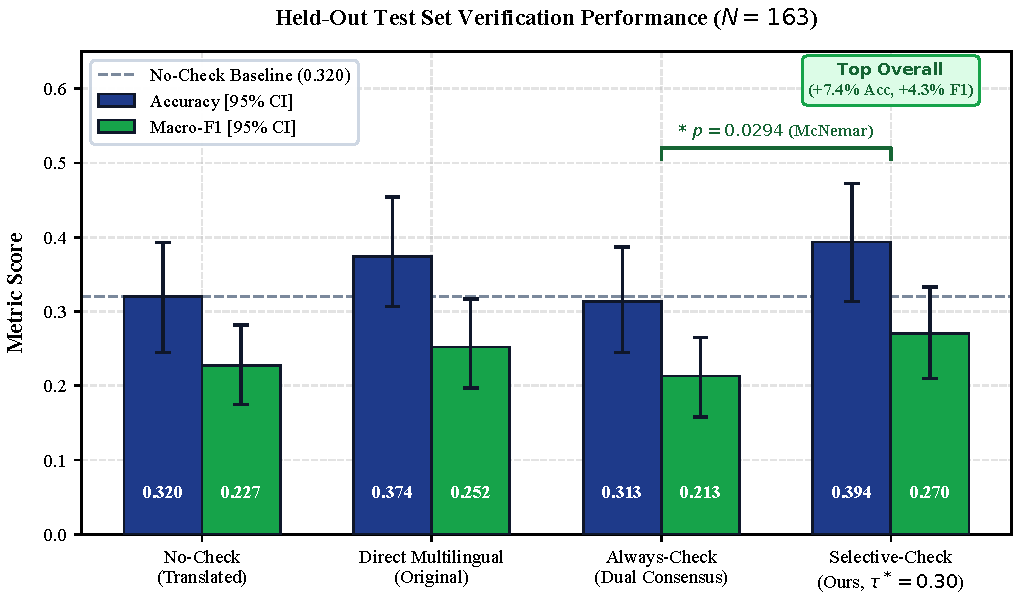
\includegraphics[width=0.98\columnwidth]{figures/pdf/fig3_condition_comparison.pdf}
\caption{Comparative performance (Accuracy and Macro-F1) across the four verification conditions on the held-out test set ($N=163$). Selective-Check achieves superior performance over naive Always-Check by avoiding negative transfer from corrupted translations.}
\label{fig:condition-comparison}
\end{figure}

Relying exclusively on machine-translated evidence (\emph{No-Check}) achieves an accuracy of 0.320 [95\% CI: 0.245, 0.393] and a Macro-F1 of 0.227 [0.175, 0.282] with a mean inference latency of 1,819.1 ms. In contrast, evaluating the original Hindi evidence directly (\emph{Direct Multilingual}) achieves an accuracy of 0.374 [0.307, 0.454] and a Macro-F1 of 0.252 [0.197, 0.317], reflecting a substantial gain of +5.4\% in accuracy and +2.5\% in Macro-F1.

Crucially, unconditional dual-language consensus (\emph{Always-Check}) achieves only 0.313 accuracy and 0.213 Macro-F1, while requiring 6,621.9 ms mean latency. This reveals a critical failure of naive consensus: when machine translation distorts factual primitives, averaging posterior probabilities forces corrupted evidence to pollute otherwise accurate original predictions. 

In contrast, our risk-calibrated \emph{Selective-Check} cascade ($\tau^*=0.300$) attains the highest performance across all conditions: \textbf{0.394} accuracy [0.313, 0.472] and \textbf{0.270} Macro-F1 [0.210, 0.333]. By preserving translated predictions when the risk trigger is low and consulting original evidence when uncertainty or numerical mismatch is elevated, Selective-Check effectively filters out corrupted translations.

\begin{table}[t]
\centering
\small
\caption{Paired statistical significance tests across conditions on test set ($N=163$). McNemar test uses discordant pair binomial calculation; permutation tests run $B=1,000$ resamples.}
\label{tab:statistical-tests}
\resizebox{\columnwidth}{!}{%
\begin{tabular}{lcccc}
\toprule
\textbf{Comparison} & \textbf{Discordant} & \textbf{McNemar $p$} & $\Delta$\textbf{F1} & \textbf{Perm. $p$} \\
\midrule
Selective-Check vs. Always-Check & 22 / 9 & \textbf{0.0294} & +0.058 & \textbf{0.0370} \\
Selective-Check vs. No-Check & 35 / 23 & 0.1480 & +0.044 & 0.1950 \\
Direct Multilingual vs. No-Check & 41 / 32 & 0.3492 & +0.026 & 0.4840 \\
\bottomrule
\end{tabular}%
}
\end{table}

\subsection{Statistical Significance}
Table~\ref{tab:statistical-tests} presents the paired statistical significance tests on the test set ($N=163$). The difference in accuracy between Selective-Check and Always-Check is statistically significant under the exact McNemar paired test ($p = 0.0294$, with 22 discordant pairs favoring Selective-Check versus only 9 favoring Always-Check). The paired permutation test ($B=1,000$) corroborates this result, showing that the Macro-F1 improvement ($\Delta\text{F1} = +0.058$) is statistically significant ($p = 0.0370$). Furthermore, Selective-Check improves over No-Check by +0.074 accuracy and +0.044 Macro-F1 ($p = 0.1480$ McNemar, 35 vs 23 discordant pairs).

\subsection{Label Flips and Discrepancy}
Across identical test items, verifier predictions flip between original and translated evidence on 102 out of 163 instances, establishing an overall \textbf{Label Flip Rate of 62.6\%} (95\% CI: [55.2\%, 69.9\%]). Among observed flips:
\begin{itemize}
    \item \textbf{Helpful Flips (41 cases, 25.2\% of all items, 40.2\% of flips):} Original evidence produces the correct ground truth while translated evidence misleads the model.
    \item \textbf{Harmful Flips (32 cases, 19.6\% of all items, 31.4\% of flips):} Translated evidence fortuitously yields the ground truth while original evidence fails.
    \item \textbf{Neutral Flips (29 cases, 17.8\% of all items, 28.4\% of flips):} Both conditions predict incorrect labels but disagree on the specific error class.
\end{itemize}

\section{Error Attribution and Qualitative Analysis}
\label{sec:errors}

\begin{table*}[t]
\centering
\small
\caption{Systematic error attribution of verification failures on the held-out test set ($N=163$). Overall Label Flip Rate between original and translated evidence is 62.6\% [55.2\%, 69.9\%] (102 / 163).}
\label{tab:error-attribution}
\begin{tabularx}{\textwidth}{lccX}
\toprule
\textbf{Error Attribution Source} & \textbf{Count} & \textbf{Share (\%)} & \textbf{Diagnostic Operational Definition} \\
\midrule
Translation-Fidelity Errors ($E_{\text{trans}}$) & 41 & 36.9\% & Factual meaning altered during translation; recovered by consulting original source. \\
Verifier-Reasoning Failures ($E_{\text{verif}}$) & 61 & 55.0\% & Verifier failed to deduce claim veracity even when original evidence was consulted. \\
Evidence Insufficiency / Ambiguity ($E_{\text{insuff}}$) & 12 & 10.8\% & Retrieved web search snippets lack sufficient factual grounding for unambiguous resolution. \\
\bottomrule
\end{tabularx}
\end{table*}

\subsection{Systematic Error Attribution}
Table~\ref{tab:error-attribution} summarizes the causal attribution of the 111 verification failures in the No-Check pipeline. Figure~\ref{fig:error-attribution} illustrates the decomposition.

\begin{figure}[t]
\centering
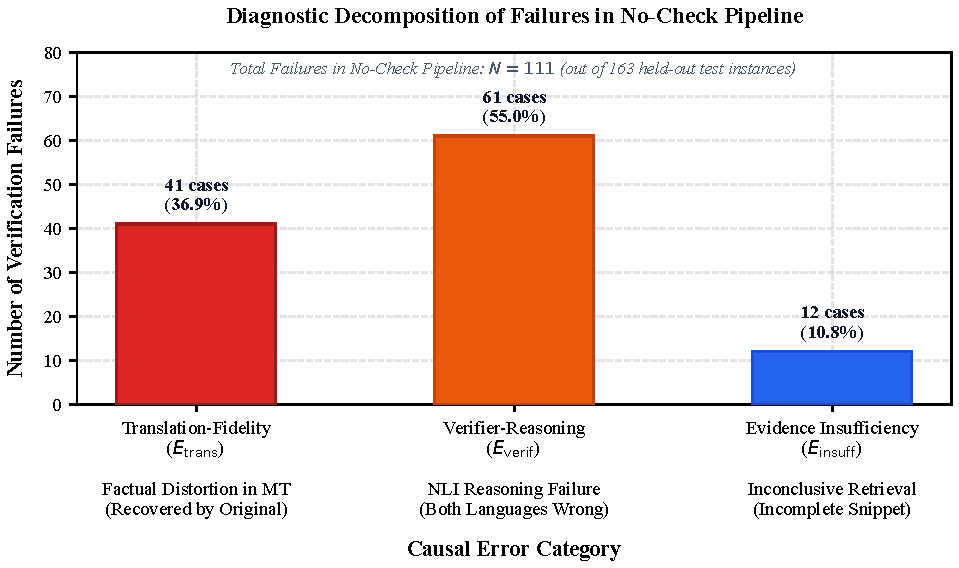
\includegraphics[width=0.98\columnwidth]{figures/pdf/fig4_error_attribution_breakdown.pdf}
\caption{Decomposition of the 111 verification failures observed in the No-Check (translated) pipeline on the test set. Translation-fidelity corruptions ($E_{\text{trans}}$) account for 36.9\% of all failures.}
\label{fig:error-attribution}
\end{figure}

\begin{itemize}
    \item \textbf{Translation-Fidelity Errors ($E_{\text{trans}}$):} Account for 41 cases (\textbf{36.9\%}). In these instances, translation corruption caused the verifier to fail, whereas consulting the original evidence restored the correct veracity label.
    \item \textbf{Verifier-Reasoning Failures ($E_{\text{verif}}$):} Account for 61 cases (\textbf{55.0\%}). Even when semantic meaning was faithfully preserved, the verifier failed to deduce the correct entailment relationship across both languages.
    \item \textbf{Evidence Insufficiency / Ambiguity ($E_{\text{insuff}}$):} Accounts for 12 cases (\textbf{10.8\%}), where retrieved web snippets were incomplete or lacked definitive grounding.
\end{itemize}

\subsection{Qualitative Case Studies}
Table~\ref{tab:case-studies} presents concrete instances illustrating the diagnostic distinctions among the three error categories.
\begin{table*}[t]
\centering
\small
\caption{Representative diagnostic case studies from the held-out test evaluation illustrating the three error categories defined in our taxonomy. Predictions reflect verdicts under No-Check ($\hat{y}_{\text{trans}}$) and Direct Multilingual ($\hat{y}_{\text{orig}}$).}
\label{tab:case-studies}
\begin{tabularx}{\textwidth}{lp{0.22\textwidth}cccX}
\toprule
\textbf{Item ID} & \textbf{Claim (English Gloss)} & \textbf{Gold} & $\hat{y}_{\text{trans}}$ & $\hat{y}_{\text{orig}}$ & \textbf{Diagnostic Failure Analysis} \\
\midrule
\texttt{hi-test-0005} & Cache of weapons seized from a mosque in Gujarat. & \textsc{Contra} & \textsc{Supp} & \textsc{Contra} & \textbf{Translation-Fidelity Error ($E_{\text{trans}}$):} Machine translation distorted fact-check context into garbled text (\emph{``Chamim f{\"u}ck welded from a moustik...''}), causing the verifier to mispredict \textsc{Supported}. Reading the original Hindi text preserved the debunking context, restoring the correct \textsc{Contradicted} verdict. \\
\addlinespace
\texttt{hi-test-0004} & Facebook CEO Mark Zuckerberg claimed ``Jai Shri Ram'' is posted 2B times daily. & \textsc{Contra} & \textsc{Supp} & \textsc{Supp} & \textbf{Verifier-Reasoning Failure ($E_{\text{verif}}$):} Machine translation faithfully preserved the viral claim and fact-check statement. However, the verifier exhibited lexical-matching bias, treating the mere mention of the viral claim in the snippet as positive entailment across both languages. \\
\addlinespace
\texttt{hi-test-0009} & 24 passengers fell ill after eating spoiled food on Tejas Express, 3 in ICU. & \textsc{Insuff} & \textsc{Supp} & \textsc{Insuff} & \textbf{Evidence Insufficiency ($E_{\text{insuff}}$):} Retrieved search snippet contained partial reporting without official medical confirmation. The original verifier abstained with \textsc{Insufficient\_Evidence}, whereas translated text induced overconfident false support. \\
\bottomrule
\end{tabularx}
\end{table*}


In item \texttt{hi-test-0005}, the original Hindi fact-check debunked a viral rumor claiming a cache of weapons had been discovered in a mosque. Neural machine translation scrambled key named entities and transliterations into disjointed phrases (\emph{``Chamim f{\"u}ck welded from a moustik...''}), causing the verifier to mispredict \textsc{Supported}. In contrast, evaluating the original Hindi text preserved the context, allowing the model to correctly identify the relation as \textsc{Contradicted}.

Conversely, item \texttt{hi-test-0004} exemplifies a verifier-reasoning failure ($E_{\text{verif}}$): although translation faithfully rendered the debunker snippet, the cross-lingual verifier was misled by lexical overlap between the viral claim and the evidence snippet, predicting \textsc{Supported} across both language representations. Finally, item \texttt{hi-test-0009} illustrates evidence insufficiency ($E_{\text{insuff}}$), where partial reporting in the search snippet provided inadequate basis for refutation, properly recognized as \textsc{Insufficient\_Evidence} under the original language pass but causing overconfident false support under translated text.

\section{Discussion and Limitations}
\label{sec:discussion}

Our results demonstrate that machine translation is not a neutral utility in cross-lingual claim verification. While translating non-English evidence into English permits standard English verifier pipelines, it imposes a 36.9\% translation error tax. Furthermore, naive dual-language consensus degrades overall accuracy because unconstrained probability averaging propagates corrupted signals into the decision. Selective checking resolves this dilemma by triggering original-evidence consultation only when predictive risk is elevated.

\textbf{Limitations:} Our study evaluates the Hindi--English language pair using MarianMT and mDeBERTa-v3 on CPU. While Hindi represents an important Indo-Aryan language with over 600 million speakers, our findings should be extended to typologically diverse language families (e.g., Dravidian, Afro-Asiatic, and Slavic languages). Additionally, error attribution was conducted on benchmark fact-checks; future work should examine human-in-the-loop expert adjudication across larger multi-hop contexts.

\section{Ethical Considerations}
\label{sec:ethics}
This study utilizes public, open-source benchmarks (X-Fact, MIT License) and locally executable open models. Automated claim verification systems must not be deployed as autonomous arbiters of truth without editorial oversight. In particular, deploying translation-dependent verification systems in low-resource linguistic communities without original-evidence safeguards risks systematically misclassifying factual evidence.

\section{Conclusion}
\label{sec:conclusion}
We presented a controlled empirical investigation decoupling translation-fidelity errors from verifier-reasoning failures in cross-lingual claim verification. On the Hindi split of the X-Fact benchmark, we uncovered a 62.6\% label flip rate between original and translated evidence, with 36.9\% of translation pipeline failures directly caused by translation corruption. By employing a risk-calibrated selective checking cascade ($\tau^*=0.300$), systems can mitigate translation-induced degradation and significantly outperform naive consensus ($p = 0.0294$).

\bibliography{references}
\bibliographystyle{acl_natbib}

\clearpage
\appendix
\section{Reproducibility Details and Hyperparameters}
\label{sec:appendix-reproducibility}

\subsection{Hardware and Compute Environment}
All experiments were conducted on a single Windows 11 workstation equipped with an AMD64 processor (18 logical cores) and 15.61~GB RAM without GPU acceleration.
\begin{itemize}
    \item \textbf{Python Environment:} Python 3.14.7, PyTorch 2.14.1 (CPU), Transformers 5.19.0.
    \item \textbf{Translation Model:} \texttt{Helsinki-NLP/opus-mt-hi-en} (parameters: 74M, beam size: 2, max length: 512). Mean translation throughput: 2.32s per evidence bundle on CPU.
    \item \textbf{Verifier Model:} \texttt{mDeBERTa-v3-base-xnli} (\texttt{MoritzLaurer/}\allowbreak\texttt{mDeBERTa-v3-base-}\allowbreak\texttt{xnli-multilingual-nli-2mil7}; parameters: 278M, sequence length: 512). Mean verification latency: 1.82s per sample on CPU.
    \item \textbf{Random Seed:} 42 for all bootstrap and permutation resamples ($B=1,000$).
\end{itemize}

\subsection{Threshold Tuning Details}
The risk threshold $\tau^*$ was tuned on the development set ($N=103$) across candidate values $\tau \in \{0.10, 0.15, \dots, 0.90\}$. The trade-off objective function was defined as:
\begin{equation}
    \mathcal{J}(\tau) = \text{Macro-F1}(\tau) - 0.15 \cdot \text{Coverage}(\tau)
\end{equation}
The optimal threshold $\tau^* = 0.300$ yielded Macro-F1 $= 0.285$, Coverage $= 0.709$, and $\mathcal{J}(\tau^*) = 0.1797$.

\subsection{Artifact and Data Availability}
All datasets, processed splits, prediction records, analysis scripts, and LaTeX manuscript sources are provided in the repository with complete execution instructions.

\end{document}
